%!TEX root = ../template.tex
%%%%%%%%%%%%%%%%%%%%%%%%%%%%%%%%%%%%%%%%%%%%%%%%%%%%%%%%%%%%%%%%%%%%
%% chapter4.tex
%% NOVA thesis document file
%%
%% Chapter with lots of dummy text
%%%%%%%%%%%%%%%%%%%%%%%%%%%%%%%%%%%%%%%%%%%%%%%%%%%%%%%%%%%%%%%%%%%%

\typeout{NT FILE chapter4.tex}%

\chapter{Related Work}
\label{cha:related_work}

\section{Schema Evolution In Serialization Frameworks} % (fold)
\label{sec:schema_evolution_in_serialization_frameworks}

Serialization is the process of encoding system state into a standardized format so that it can be delivered across a network or stored with durability.
For serialization, each language usually provides a corresponding library, such as Java serialization.
In the setting of service oriented architectures, serialization libraries supplied by programming languages are typically not used to encode messages between services,
because each service may be written in a different language. As a result, data consumers will be unable to comprehend data producers.
Cross-language serialization libraries, such as JSON, can solve this problem.
However, formats such as JSON lack a strictly defined structure,
making data consumption more difficult due to poor type-safety guarantees, and the ability for fields to be unilaterally added or withdrawn at any moment without the consumers' knowledge.
What's missing is a "schema" for data exchange between producers and consumers, akin to an API contract.

There have been a few cross-language serialization libraries that require the data structure to be properly described via schemas.
XML, Avro, Thrift, and Protocol Buffers are among these libraries.
The benefit of having a schema is that it explicitly defines the data's structure, type, and meaning (through documentation).

Such libraries allow for schema evolution (adding fields, deleting fields, and renaming fields) [24, 25], but only to a limited extent:
\begin{itemize}
    \item To ensure backwards compatibility, added fields must be optional.
    \item The only fields that can be removed to maintain forward compatibility are optional fields.
    \item To provide both forward and backward compatibility, removed and new fields must be optional.
\end{itemize}
Backward comparability refers to a consumer using schema X to process data produced by schema X-1,
whereas forward compatibility refers to data produced by schema X being read by consumers using schema X-1.
These limitations are problematic because, in order to enforce required fields, validation logic would need to be written repeatedly by programmers (in the same layer as the business logic).
The scale of the validation logic is proportional to the complexity of messages being validated;
for messages with more properties, particularly those with nested objects, the validation footprint can rise dramatically in terms of both line-count and logical complexity.

In Avro there are also additional limitations in the ability to rename fields due to the way data is encoded and translated across schemas.

\begin{figure}[htbp]
    \centering
    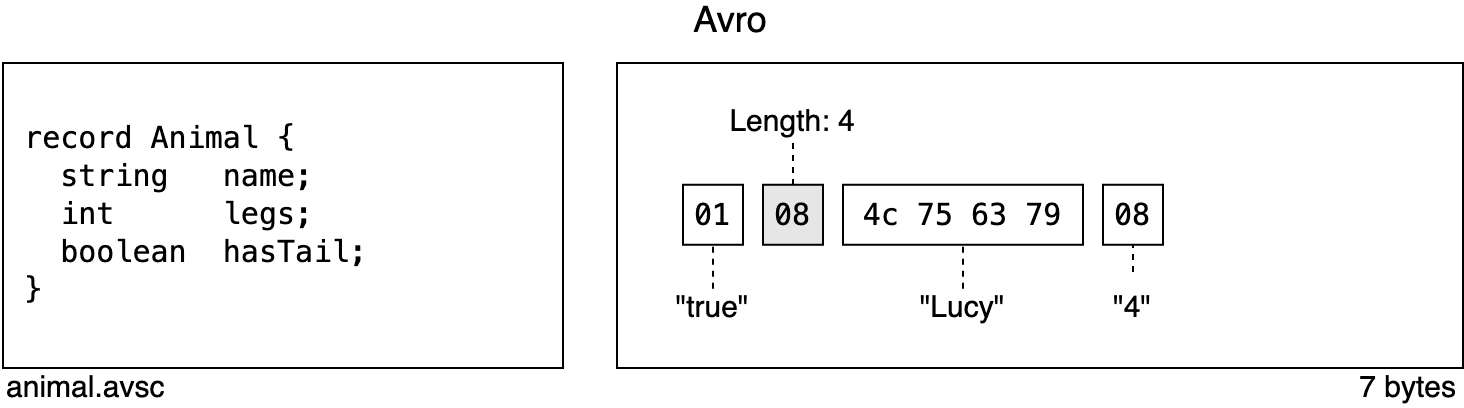
\includegraphics[height=1.5in]{avro}
    \caption{Imagem em formato \emph{bitmap} (JPG)}
    \label{fig:Figuras_Tree_silhouettes-bitmap}
\end{figure}

On the left-hand side, you can see a Avro schema for the type “Animal” with the three fields “name”, “legs” and “hasTail”, respectively. On the right hand side, you can see a record which was serialized with that schema. We easily find that the animal in question is named “Lucy”, has four legs and a tail. You don’t have to understand every detail of the binary output, just know that the tags (marked in orange) tell the deserializer which bytes correspond to which field. This is important because the fields in the byte sequence are not in the same order as they were defined in the schema.

Instead, in the serialized byte sequence, all fields are appended back to back.

\begin{figure}[htbp]
    \centering
    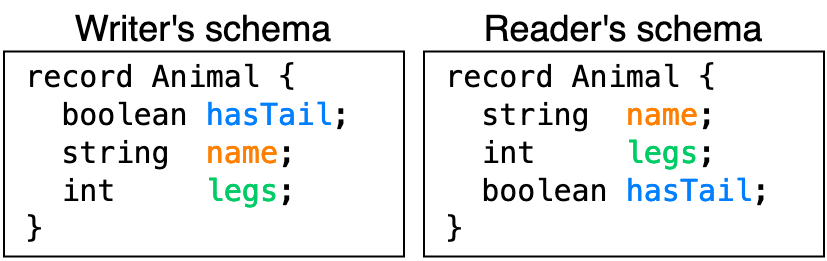
\includegraphics[height=1.5in]{avro-side}
    \caption{Imagem em formato \emph{bitmap} (JPG)}
    \label{fig:Figuras_Tree_silhouettes-bitmap}
\end{figure}

\begin{figure}[htbp]
    \centering
    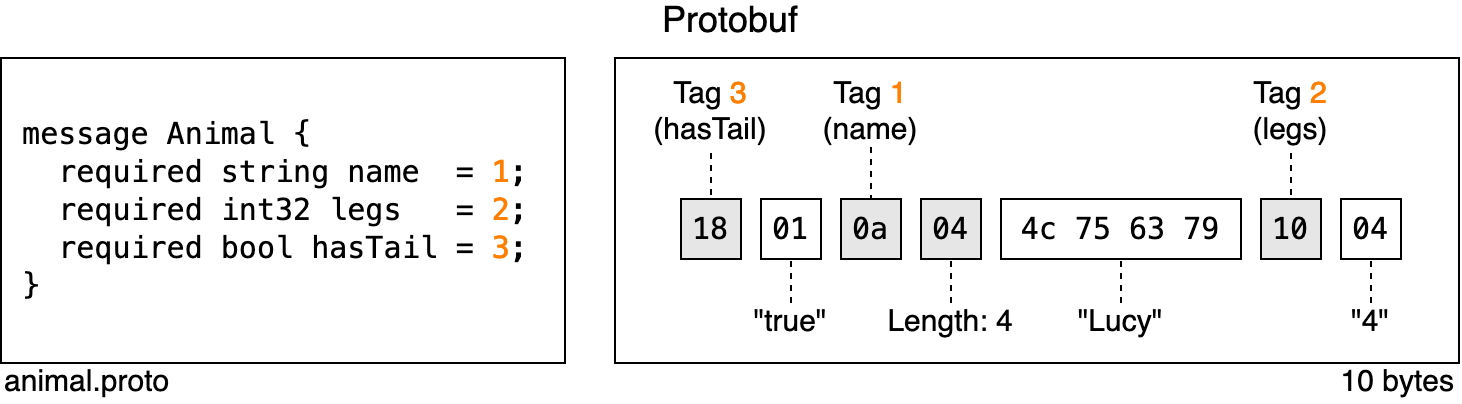
\includegraphics[height=1.5in]{protobuf}
    \caption{Imagem em formato \emph{bitmap} (JPG)}
    \label{fig:Figuras_Tree_silhouettes-bitmap}
\end{figure}

These frameworks only tackle part of the problem of API evolution in microservices,
because they can only accommodate changes in the schema of parameters.
They can not manage changes in the API's signature, such as the method of a REST endpoint.
To eliminate potential mismatches and reduce the complexity of the evolution process, we believe it is critical to manage both sorts of evolution's in a single integrated approach.

\section{Service Integration Adapters} % (fold)
\label{sec:service_integration_adapters}

In the context of service-oriented architectures (SOA) there has been extensive
research on the adaptability of services [3, 4, 6, 7, 14, 27]. There are similarities
between SOA and microservices, as both follow a separation of concerns approach
based on services. These two architectures diverge on some relevant features, in
particular on the fact the SOA services are tightly-coupled while microservices are
loosely-coupled. As a consequence, adaptability in SOA is not focused on evolution
but on the integration of microservices. These works [3, 4, 7, 14, 27] on SOA address
and develop adapters for behavioural mismatches among business processes. The
concern is mainly on adapting workflows and most assume that data adaptation is
already defined by developers. Standard service binding technologies (cf. SOAP) use
description languages like WSDL [1] to specify contracts, allowing them to check for
compatibility of services on every remote call, and issue runtime exceptions when some
mismatch happens. Schema registries and service brokers are also used to centralize
10:27
Robust Contract Evolution in a TypeSafe MicroService Architectures
and authorise changes in the service architecture. Schemas can then be checked based
on version identifiers and compatibility relations just like in our case [22].

\section{Chain Adapter} % (fold)
\label{sec:chain_adapter}

\section{Deployment Strategies} % (fold)
\label{sec:deployment_strategies}

\section{Schema Registry} % (fold)
\label{sec:schema_registry}
